% !TEX program = xelatex
\documentclass[a4paper,10pt]{article}
\usepackage{amsthm}
\usepackage{amssymb}
\usepackage{bm}
\usepackage{mathtools}
\usepackage[x11names]{xcolor}
\usepackage{xparse}
\usepackage{fontspec}
\usepackage{unicode-math}
\setromanfont[Ligatures={Common,Rare}]{DovesType-Regular.otf}
\setsansfont{Andika}
\setmathfont{Asana Math}[Scale=1]
\newfontfamily\TrajanP[Scale=1.0]{TRAJANPRO-REGULAR.OTF}
% \newfontfamily\TrajanP[Scale=1.0]{Tork}

% \usepackage{pstricks}
\usepackage{varwidth}
\usepackage{siunitx}
\usepackage{graphicx}
\usepackage[margin=1.5cm,top=1.5cm]{geometry}
\usepackage[most]{tcolorbox}
\usepackage{pgfplots}
\pgfplotsset{compat=newest}
\tcbuselibrary{skins,xparse,poster,breakable}
% \usetikzlibrary{fadings}
\usetikzlibrary{calc,math, plotmarks, shapes, shapes.geometric, positioning, angles, intersections, quotes, through, patterns, turtle, arrows.meta}
\usetikzlibrary{decorations.markings,backgrounds}
% \usepackage{etoolbox}
\usepackage{tkz-euclide}
\usepackage{xfrac}
% \usepackage{xlop}
% \newcommand\hole[2]{#1}  % for use with xlop
\pagenumbering{gobble}
%%%%%%%%%%%%%%%%%%%%%%%%%%%%%%%%%%%%%%%%%%%%%%%%%%%%%%%%%
\newcommand\markangle[9]{% origin X Y radius radiusmark mark colour opacity
%  % fill red circle offset-from-centre
  \begin{scope}
    \path[clip] (#1) -- (#2) -- (#3);
    \fill[color=#7,fill opacity=#8,draw=black,name path global=pcircle]  % global declaration required otherwise pcircle is not seen by the `named intersections=' lines below.
    (#1) circle (#4);
  \end{scope}
  % middle calculation
  \path[name path=line one] (#1) -- (#2);
  \path[name path=line two] (#1) -- (#3);
  \path[%
  name intersections={of=line one and pcircle, by={inter one}},
  name intersections={of=line two and pcircle, by={inter two}}
  ] (inter one) -- (inter two) coordinate[pos=#9] (place);
  % put mark
  \node at ($(#1)!#5!(place)$) {\scriptsize{#6}};
}
%%%%%%%%%%%%%%%%%%%%%%%%%%%%%%%%%%%%%%%%%%%%%%%%%%%%%%%%
\newcommand\tcircle[6]{% centre coord (x,y), radius, points, radpoint, colour, edge
  \coordinate (O) at (#1,#2); % centre of the circle
  \def\radius{#3}          % radius of the circle
  \def\npts{#4}            % number of the points
  \def\radpt{#5}           % radius of the points
  \colorlet{ptcolour}{#6}  % colour of the points
  % \draw (O) circle (\radius);
  \foreach \numpoint in {1,...,\npts}{
    \fill[ptcolour] (O) ++ (360/\npts*\numpoint:\radius) coordinate (C\numpoint) circle(\radpt);
  }
}

% \newcommand{\condSoln}[2]{\ifcsdef{r@#1}{#2}{}}

% \newcommand\fadingtext[3][]{%
%    \begin{tikzfadingfrompicture}[name=fading letter]
%      \node[text=transparent!0,inner xsep=0pt,outer xsep=0pt,#1] {#3};
%    \end{tikzfadingfrompicture}%
%    \begin{tikzpicture}[baseline=(textnode.base)]
%      \node[inner sep=0pt,outer sep=0pt,#1](textnode){\phantom{#3}};
%      \shade[path fading=fading letter,#2,fit fading=false]
%      (textnode.south west) rectangle (textnode.north east);%
%    \end{tikzpicture}%
% }

\definecolor{JISpurple}{RGB}{89,72,122}
\definecolor{JISivory}{RGB}{241,234,221}
\definecolor{JIStaupe}{RGB}{183,156,154}
\definecolor{PaleGreen}{RGB}{240,255,240} % 'Honeydew'

\AddToHook{shipout/background}{%
    \put (0in,-\paperheight){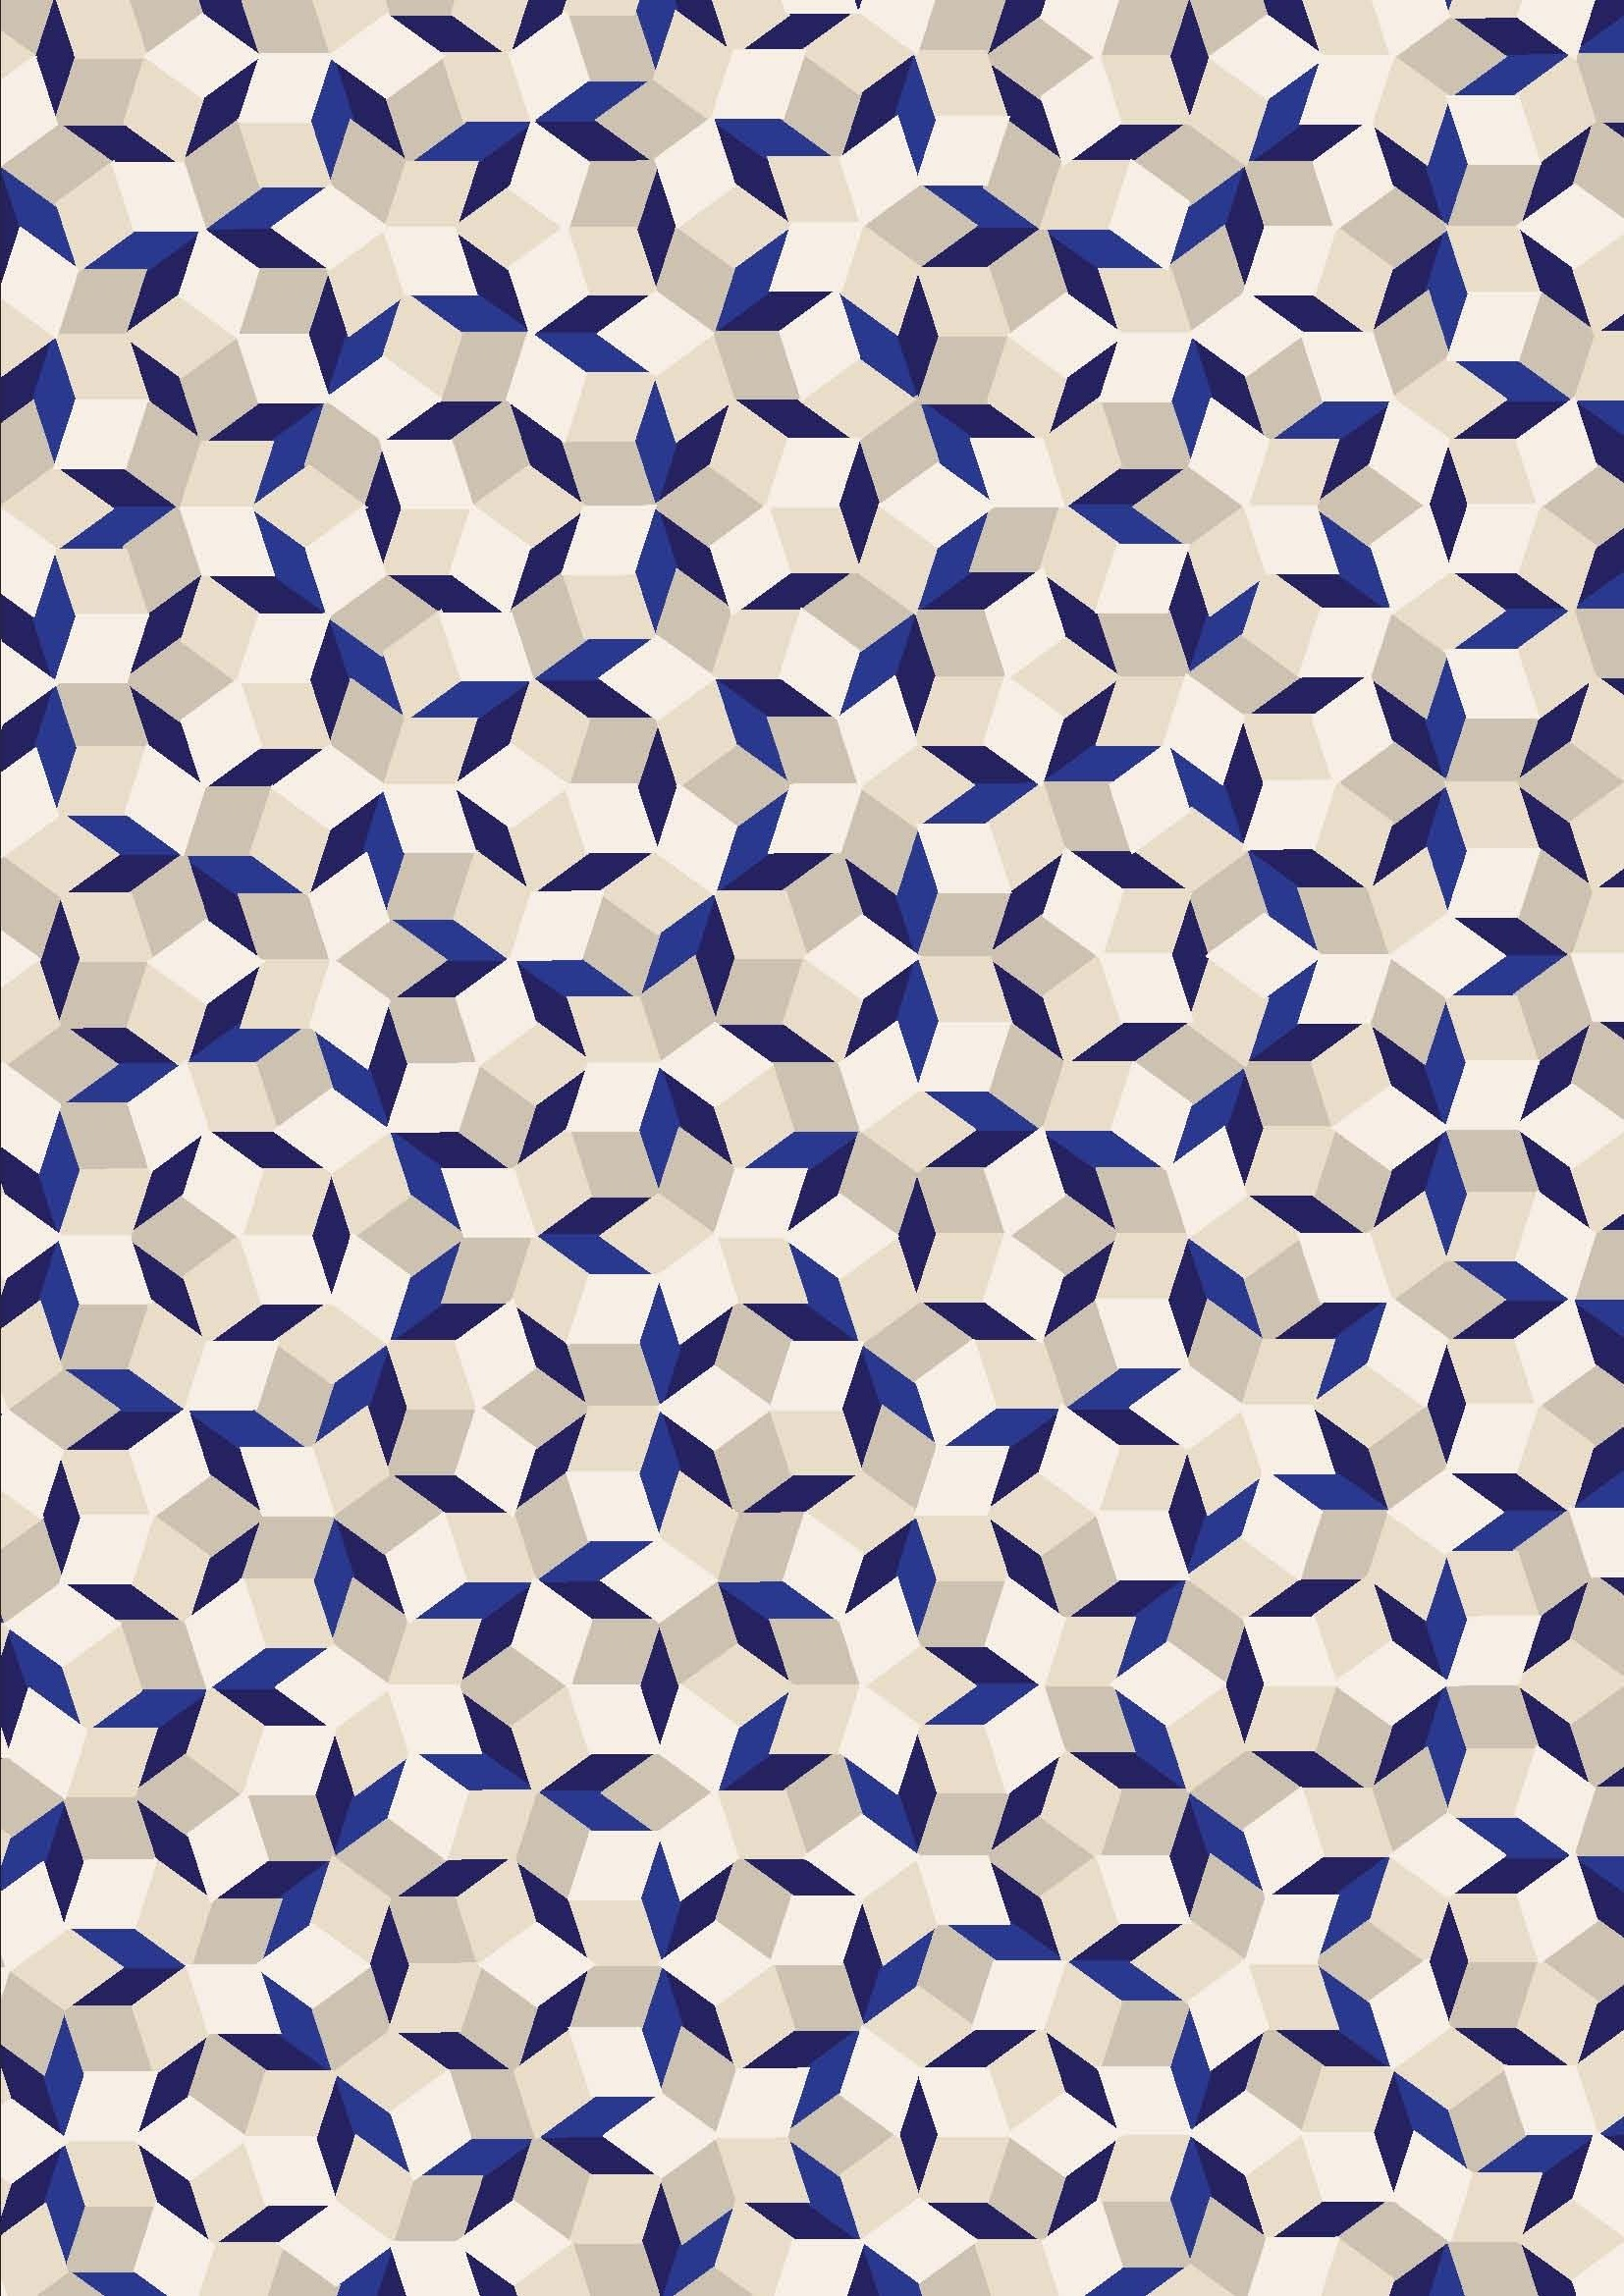
\includegraphics[width=\paperwidth,height=\paperheight]{images/penrose2r.jpg}}%
}

\newcommand\numberthis{\addtocounter{equation}{1}\tag{\theequation}}

\newtcolorbox{MyOuterBox}{%
  enhanced,
  % watermark graphics=images/santa_faces_watermark.jpg,
  % watermark opacity=0.8,
  % watermark zoom=2.0,
  breakable,
  frame style=JISpurple,
  colback=JISivory,
  colframe=JISpurple,
  title={
\includegraphics[width=0.9cm,height=0.9cm]{images/JIS Final Logo FA-02.png}\raisebox{3mm}{\Large{Maths Challenge}\hspace{24.0em} \Large{\bfseries\sffamily 24}}},
}

\newtcolorbox{MyInnerBox}[2][]{enhanced,%empty,
coltitle=JISpurple,colback=white,
breakable,
fonttitle=\bfseries\sffamily,
attach boxed title to top left={yshift=-1.5mm},
boxed title style={empty, size=small, top=1mm, bottom=0pt},
varwidth boxed title=0.5\linewidth,
frame code={
  \path (title.east|-frame.north) coordinate (aux);
\path[draw=JISpurple, line width=0.5mm, rounded corners,fill=white]
(frame.west) |- ([xshift=-2.5mm]title.north east) to[out=0, in=180] ([xshift=7.5mm]aux)-|(frame.east)|-(frame.south)-|cycle;
},
title={#2},#1}

\newtcolorbox{MyInnerSplitBox}[2][]{enhanced,%empty,
bicolor,sidebyside,sidebyside align=top seam,
righthand width=7.0cm,colbacklower=white,
sidebyside gap=5mm,
breakable,
coltitle=JISpurple,colback=white,
fonttitle=\bfseries\sffamily,
attach boxed title to top left={yshift=-1.5mm},
boxed title style={empty, size=small, top=1mm, bottom=0pt},
varwidth boxed title=0.5\linewidth,
frame code={
  \path (title.east|-frame.north) coordinate (aux);
\path[draw=JISpurple, line width=0.5mm, rounded corners,fill=white]
(frame.west) |- ([xshift=-2.5mm]title.north east) to[out=0, in=180] ([xshift=7.5mm]aux)-|(frame.east)|-(frame.south)-|cycle;
},
title={#2},#1}


\newtcolorbox{MySolutionBox}[1][]{%
  enhanced,
  breakable,
  frame style=JISpurple,
  colback=PaleGreen, colframe=green,
  title={\Large Solution},
  drop fuzzy shadow,
  halign=left,
  #1
}

%%%%%%%%%%%%%%%%%%%%%%%%%%%%%%%%%%%%%%%%%%%%%%%%%%
\newtoggle{SOLUTION}
%%% Uncomment the appropriate line below to show solutions %%%
% \toggletrue{SOLUTION}
\togglefalse{SOLUTION}
%%%%%%%%%%%%%%%%%%%%%%%%%%%%%%%%%%%%%%%%%%%%%%%%%


%%%%%%%%%%%%%%%%%%%%%%%%%%%%%%%%%%%%%%%%%%%%%%%%%%
%%%%%%            DOCUMENT BEGINS           %%%%%%
%%%%%%%%%%%%%%%%%%%%%%%%%%%%%%%%%%%%%%%%%%%%%%%%%%
\begin{document}


  \begin{MyOuterBox}
    \iftoggle{SOLUTION}{Here are the full, or partial solutions.
    }{
      Welcome to this week's Maths Challenge!\\
      Have a go at all three questions!\\
      Drop your solution in the box in the staffroom by Tuesday.
    }
       \begin{MyInnerBox}{All years, question 1}
     Welcome to the third installment of Portia's Caskets! This time, Portia tells you that every casket has been made by one of two famous Florentine craftsmen, Bellini and Cellini. She explains that Cellini always writes a false statement on the lids of the caskets he makes, while Bellini only puts true statements on the lids of the  caskets he builds. As before, Portia is truthful.\par
     For this first puzzle, Portia tells you that she has hidden a dagger in one of the caskets. To pass this test, you must avoid choosing the casket with the dagger.\par\vspace{3mm}
     \begin{tikzpicture}[scale=0.8,font=\fontfamily{TrajanP}\selectfont]
          \path[draw,line width=3mm,DarkGoldenrod1,fill overzoom image=images/wp7316403.jpg] (1,1.5) to[bend left=45] (1.5,1) -- (6.5,1) to[bend left=45] (7,1.5) -- (7,6.5) to[bend left=45] (6.5,7)-- (1.5,7) to[bend left=45] (1,6.5) -- cycle;
          \path[draw,line width=0.5mm,DarkGoldenrod4] (1.4,1.9) to[bend left=45] (1.9,1.4) -- (6.1,1.4) to[bend left=45] (6.6,1.9) -- (6.6,6.1) to[bend left=45] (6.1,6.6)-- (1.9,6.6) to[bend left=45] (1.4,6.1) -- cycle;
          \path[fill overzoom image=images/goldbrush.jpg] (2.0,2.0) -- (6.0,2.0) -- (6.0,6.0) -- (2.0,6.0) -- cycle;
          \node[black,align=center,text width=4cm] at (4,4.2) {\baselineskip=15pt\TrajanP The dagger\\\TrajanP is in\\\TrajanP this casket.\par};
        \end{tikzpicture}\hspace{2mm}
        \begin{tikzpicture}[scale=0.8]
          \path[draw,line width=3mm,Snow2,fill overzoom image=images/SilverFoil.jpg] (1,1.5) to[bend left=45] (1.5,1) -- (6.5,1) to[bend left=45] (7,1.5) -- (7,6.5) to[bend left=45] (6.5,7)-- (1.5,7) to[bend left=45] (1,6.5) -- cycle;
          \path[draw,line width=0.5mm,white] (1.4,1.9) to[bend left=45] (1.9,1.4) -- (6.1,1.4) to[bend left=45] (6.6,1.9) -- (6.6,6.1) to[bend left=45] (6.1,6.6)-- (1.9,6.6) to[bend left=45] (1.4,6.1) -- cycle;
          \path[fill overzoom image=images/silverBg.jpg] (2.0,2.0) -- (6.0,2.0) -- (6.0,6.0) -- (2.0,6.0) -- cycle;
          \node[black,align=center,text width=4cm] at (4,4.2) {\baselineskip=12pt\TrajanP  This casket \\\TrajanP is empty.\par};
        \end{tikzpicture}\hspace{2mm}
        \begin{tikzpicture}[scale=0.8]
          \path[draw,line width=3mm,SlateGray4,fill overzoom image=images/LeadBg.jpg] (1,1.5) to[bend left=45] (1.5,1) -- (6.5,1) to[bend left=45] (7,1.5) -- (7,6.5) to[bend left=45] (6.5,7)-- (1.5,7) to[bend left=45] (1,6.5) -- cycle;
          \path[draw,line width=0.5mm,black] (1.4,1.9) to[bend left=45] (1.9,1.4) -- (6.1,1.4) to[bend left=45] (6.6,1.9) -- (6.6,6.1) to[bend left=45] (6.1,6.6)-- (1.9,6.6) to[bend left=45] (1.4,6.1) -- cycle;
          \path[fill=Ivory3,opacity=0.3] (2.0,2.0) -- (6.0,2.0) -- (6.0,6.0) -- (2.0,6.0) -- cycle;
          \node[black,align=center,text width=4cm] at (4,4.2) {\baselineskip=15pt\TrajanP At most one \\\TrajanP of these \\\TrajanP three caskets\\\TrajanP was fashioned\\\TrajanP by Bellini.\par};
        \end{tikzpicture}
      \iftoggle{SOLUTION}{%conditional output begin
      \begin{MySolutionBox}
        We consider each container in turn, first assuming it was made by Bellini and checking for logical consistency, then assuming it was made by Cellini and checking again.\par
        Let's start with the lead casket as it looks like it will give more information:\par
        \underline{Case 1: The lead casket was made by Bellini}\par
        \hspace{1em} The statement on the lead casket is true, and therefore the gold and silver caskets must have been manufactured by Cellini and thus have false statements on their lids.\par
        \hspace{1em}The gold statement is a lie, the dagger is not in the gold casket. The silver statement is also a lie and so the dagger is in the silver casket.\par
        There is no contradiction here, the dagger could be in the silver box.\par\medskip
        \underline{Case 2: The lead casket was made by Cellini}\par
        \hspace{1em} The statement of the lead casket is false, and therefore two of the caskets must have been fashioned by Bellini, not the lead one, so the gold and silver caskets must have true statements.\par
        \hspace{1em} The gold statement is true so the dagger is in the gold box. The silver statement is also true and so the dagger is not in the silver casket.\par
        There is no contradiction here, the dagger could be in the gold box.\par\medskip
        The dagger could be in the gold or silver caskets, so we choose the lead one.\par\medskip
      \end{MySolutionBox}
    }{}%conditional output end
    \end{MyInnerBox}


    \vspace{0.4cm}
          \begin{MyInnerBox}{All years, question 2}
        In this test, Portia places a portrait of herself in one of only two caskets, there are no daggers. As in the first puzzle, each casket is made by either Cellini or Bellini.\par
        Which casket holds Portia's portrait?\par\vspace{3mm}
        \begin{tikzpicture}[scale=0.8,font=\fontfamily{TrajanP}\selectfont]
          \path[draw,line width=3mm,DarkGoldenrod1,fill overzoom image=images/wp7316403.jpg] (1,1.5) to[bend left=45] (1.5,1) -- (6.5,1) to[bend left=45] (7,1.5) -- (7,6.5) to[bend left=45] (6.5,7)-- (1.5,7) to[bend left=45] (1,6.5) -- cycle;
          \path[draw,line width=0.5mm,DarkGoldenrod4] (1.4,1.9) to[bend left=45] (1.9,1.4) -- (6.1,1.4) to[bend left=45] (6.6,1.9) -- (6.6,6.1) to[bend left=45] (6.1,6.6)-- (1.9,6.6) to[bend left=45] (1.4,6.1) -- cycle;
          \path[fill overzoom image=images/goldbrush.jpg] (2.0,2.0) -- (6.0,2.0) -- (6.0,6.0) -- (2.0,6.0) -- cycle;
          \node[black,align=center,text width=4cm] at (4,4.2) {\baselineskip=15pt\TrajanP The \textbf{Portrait} \\\TrajanP is not in this\\\TrajanP casket.\par};
        \end{tikzpicture}\hspace{2mm}
        \begin{tikzpicture}[scale=0.8]
          \path[draw,line width=3mm,Snow2,fill overzoom image=images/SilverFoil.jpg] (1,1.5) to[bend left=45] (1.5,1) -- (6.5,1) to[bend left=45] (7,1.5) -- (7,6.5) to[bend left=45] (6.5,7)-- (1.5,7) to[bend left=45] (1,6.5) -- cycle;
          \path[draw,line width=0.5mm,white] (1.4,1.9) to[bend left=45] (1.9,1.4) -- (6.1,1.4) to[bend left=45] (6.6,1.9) -- (6.6,6.1) to[bend left=45] (6.1,6.6)-- (1.9,6.6) to[bend left=45] (1.4,6.1) -- cycle;
          \path[fill overzoom image=images/silverBg.jpg] (2.0,2.0) -- (6.0,2.0) -- (6.0,6.0) -- (2.0,6.0) -- cycle;
          \node[black,align=center,text width=4cm] at (4,4.2) {\baselineskip=15pt\TrajanP Exactly one \\\TrajanP of these two \\\TrajanP caskets was\\\TrajanP fashioned by\\\TrajanP Bellini.\par};
        \end{tikzpicture}
      \iftoggle{SOLUTION}{%conditional output begin
      \begin{MySolutionBox}
        Again, we will assume that one of the caskets is made by Bellini, and again we will begin with the casket that looks like it will provide more information. In this case, the silver one.\par
        \underline{Case 1: The silver casket was made by Bellini}\par
        \hspace{1em} The silver box has a true statement as it was made by Bellini. From this silver statement, the gold casket must have been made by Cellini.\par
        \hspace{1em} The statement on the gold box is false, so the portrait is inside.\par
        We could just stop here, we have found a logically consistent answer, and if the problem is well-formed, the other case should lead to the same conclusion.\par\medskip
        \underline{Case 2: The silver casket was made by Cellini}\par
        \hspace{1em} The statement on the silver box is false, so both caskets were made by Cellini.\par
        \hspace{1em} The statement on the gold box is false, so the portrait is inside.\par
        This case leads to the same conclusion, the portrait is in the gold casket.\par\medskip
      \end{MySolutionBox}
    }{}%conditional output end
    \end{MyInnerBox}


    \vspace{0.4cm}
          \begin{MyInnerBox}{All years, question 3}
        Again each of the caskets has been fashioned either by Bellini or Cellini. Portia has again placed a portrait of herself in one of the three boxes. This time, to win the prize (a moment of inspiration on a foggy day) you must find the portrait and tell the maker of each casket.\par\vspace{3mm}
        \begin{tikzpicture}[scale=0.8,font=\fontfamily{TrajanP}\selectfont]
          \path[draw,line width=3mm,DarkGoldenrod1,fill overzoom image=images/wp7316403.jpg] (1,1.5) to[bend left=45] (1.5,1) -- (6.5,1) to[bend left=45] (7,1.5) -- (7,6.5) to[bend left=45] (6.5,7)-- (1.5,7) to[bend left=45] (1,6.5) -- cycle;
          \path[draw,line width=0.5mm,DarkGoldenrod4] (1.4,1.9) to[bend left=45] (1.9,1.4) -- (6.1,1.4) to[bend left=45] (6.6,1.9) -- (6.6,6.1) to[bend left=45] (6.1,6.6)-- (1.9,6.6) to[bend left=45] (1.4,6.1) -- cycle;
          \path[fill overzoom image=images/goldbrush.jpg] (2.0,2.0) -- (6.0,2.0) -- (6.0,6.0) -- (2.0,6.0) -- cycle;
          \node[black,align=center,text width=4cm] at (4,4.2) {\baselineskip=15pt\TrajanP The \textbf{Portrait} \\\TrajanP is in here.\par};
        \end{tikzpicture}\hspace{2mm}
        \begin{tikzpicture}[scale=0.8]
          \path[draw,line width=3mm,Snow2,fill overzoom image=images/SilverFoil.jpg] (1,1.5) to[bend left=45] (1.5,1) -- (6.5,1) to[bend left=45] (7,1.5) -- (7,6.5) to[bend left=45] (6.5,7)-- (1.5,7) to[bend left=45] (1,6.5) -- cycle;
          \path[draw,line width=0.5mm,white] (1.4,1.9) to[bend left=45] (1.9,1.4) -- (6.1,1.4) to[bend left=45] (6.6,1.9) -- (6.6,6.1) to[bend left=45] (6.1,6.6)-- (1.9,6.6) to[bend left=45] (1.4,6.1) -- cycle;
          \path[fill overzoom image=images/silverBg.jpg] (2.0,2.0) -- (6.0,2.0) -- (6.0,6.0) -- (2.0,6.0) -- cycle;
          \node[black,align=center,text width=4cm] at (4,4.2) {\baselineskip=15pt\TrajanP The \textbf{Portrait} \\\TrajanP is in here.\par};
        \end{tikzpicture}\hspace{2mm}
        \begin{tikzpicture}[scale=0.8]
          \path[draw,line width=3mm,SlateGray4,fill overzoom image=images/LeadBg.jpg] (1,1.5) to[bend left=45] (1.5,1) -- (6.5,1) to[bend left=45] (7,1.5) -- (7,6.5) to[bend left=45] (6.5,7)-- (1.5,7) to[bend left=45] (1,6.5) -- cycle;
          \path[draw,line width=0.5mm,black] (1.4,1.9) to[bend left=45] (1.9,1.4) -- (6.1,1.4) to[bend left=45] (6.6,1.9) -- (6.6,6.1) to[bend left=45] (6.1,6.6)-- (1.9,6.6) to[bend left=45] (1.4,6.1) -- cycle;
          \path[fill=Ivory3,opacity=0.3] (2.0,2.0) -- (6.0,2.0) -- (6.0,6.0) -- (2.0,6.0) -- cycle;
          \node[black,align=center,text width=4cm] at (4,4.2) {\baselineskip=15pt\TrajanP At least \\\TrajanP two of these\\\TrajanP caskets were\\\TrajanP fashioned by\\\TrajanP Cellini.\par};
        \end{tikzpicture}
      \iftoggle{SOLUTION}{%conditional output begin
      \begin{MySolutionBox}
        We start by noticing the lead casket gives most information about the caskets:\par
        \underline{Case 1: The lead casket was made by Bellini}\par
        \hspace{1em} The statement on the lead box is true, this means that the gold and silver containers were made by Cellini.\par
        \hspace{1em}Both the gold and silver statements are false. No contradictions. The portrait must be in the lead box and we have Gold: Cellini, Silver: Cellini, Lead: Bellini.\par\medskip
        \underline{Case 2: The lead casket was made by Cellini}\par
        \hspace{1em} The statement on the lead box is false. At most one of the caskets was made by Cellini.\par
        \hspace{1em} Since we assumed the lead box was made by Cellini, the gold and silver caskets must have been made by Bellini, which means the statements on both are true.\par
        \hspace{1em} But this leads to an inconsistency since both boxes claim to contain the portrait.\par
        This case leads to an contradiction, Case 2 cannot be correct.\par\medskip
        So we have confirmed Case 1: The portrait must be in the lead box and the gold and silver caskets were made by Cellini, while the lead casket was made by Bellini.\par\medskip
      \end{MySolutionBox}
    }{}%conditional output end
    \end{MyInnerBox}


  \end{MyOuterBox}

%%%%%%%%%%%%%%%%%%%%%%%%%%%%%%%%%%%%%%%%%%%%%%%%%%
\end{document}



